%!TEX root = uber.tex

\section{Robustness of Strategies}
\begin{frame}{Robust Earnings Problem}
	\only<1>{
	\begin{figure}
	\centering
	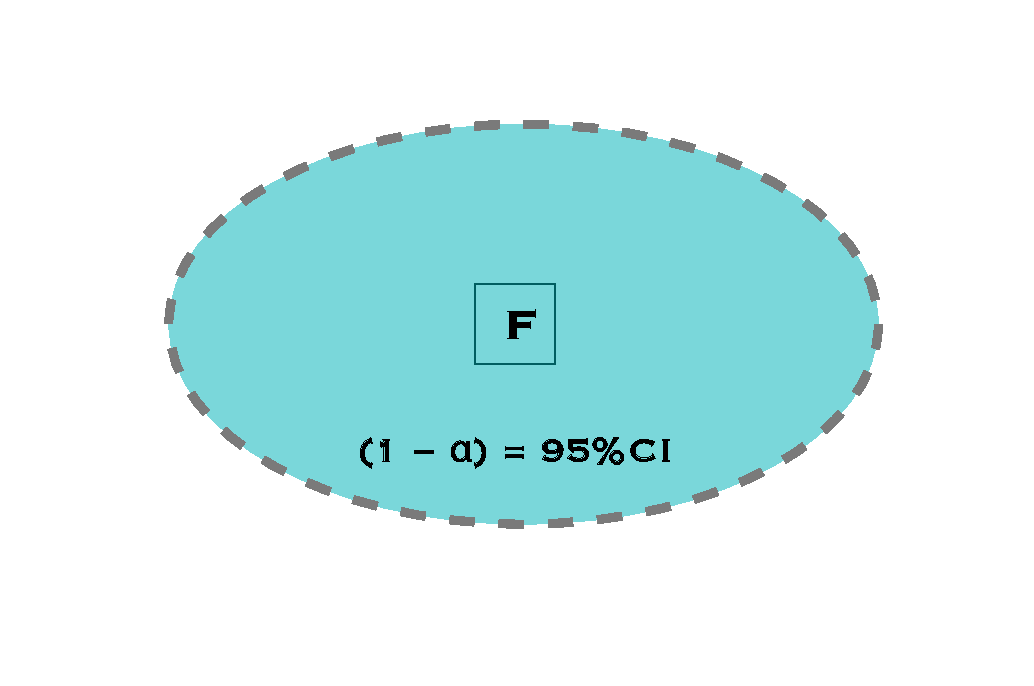
\includegraphics[scale=0.20]{figures/robustness.pdf}
	% \caption{Effect of uncertainty}
	\end{figure}
	}
	\only<2>{
	\begin{figure}
	\centering
	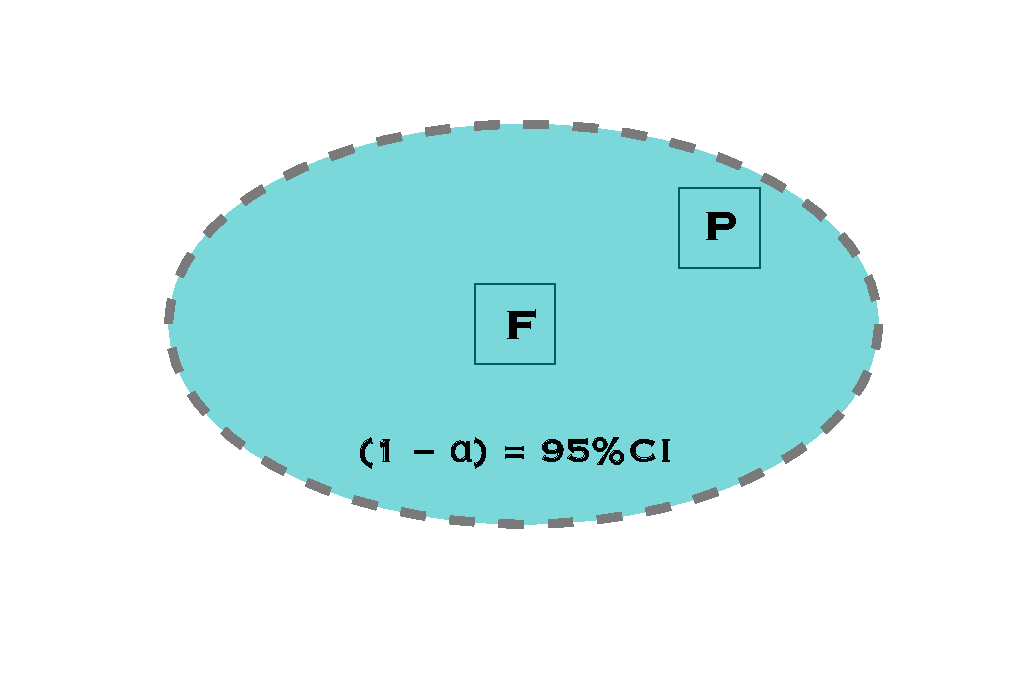
\includegraphics[scale=0.20]{figures/robustness1.pdf}
	% \caption{Effect of uncertainty}
	\end{figure}
	}
	\uncover<3->{
	\begin{figure}
	\centering
	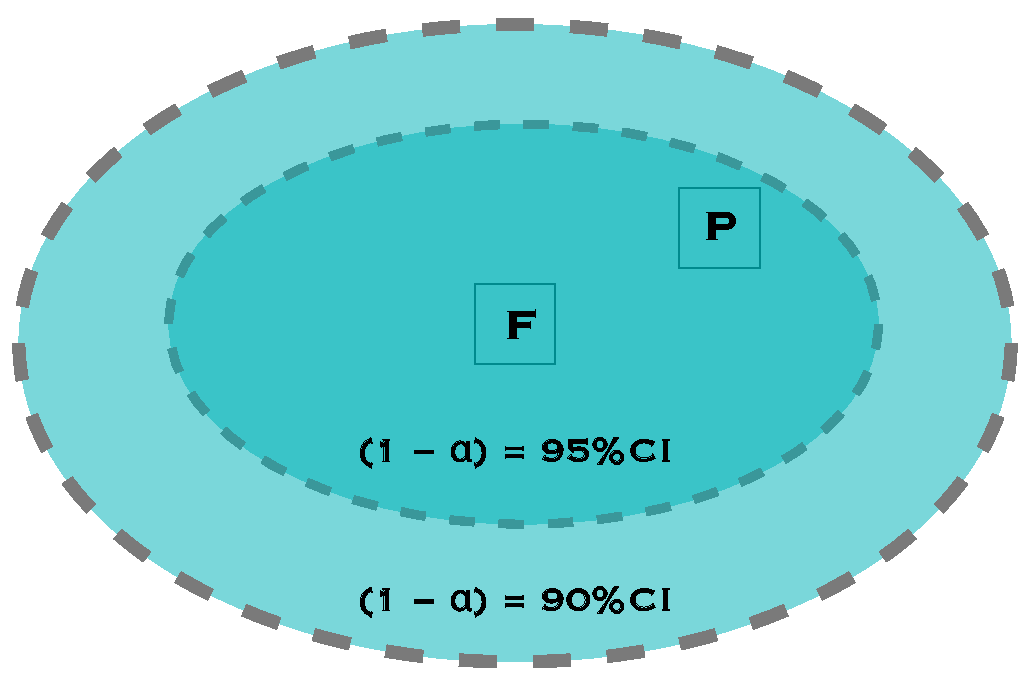
\includegraphics[scale=0.20]{figures/robustness2.pdf}
	% \caption{Effect of uncertainty}
	\end{figure}
	}
	\uncover<4->{
	\begin{itemize}
		%\item Strategies can be very sensitive to changes in transition matrices.
		%\pause
		\item $\mathcal{P}_\alpha$: set of transition matrices within $(1-\alpha)$ CI of observed $F$ i.e. $\alpha$ uncertainty.
	\end{itemize}
	}
\uncover<5->{
\textbf{\textsc{RobustEarnings Problem}:} Find a policy $\pi^\ast$ such that:
\begin{equation*}
\pi^\ast = \argmax_{\pi \in \Pi} \min_{P \in \mathcal{P}_\alpha} \mathcal{E}(\pi, P, T, R, B). 
\end{equation*}
}
\uncover<6->{\alert{\textcite{nilim2004robustness}: DP augmented with an optimization step, solvable in polynomial time.}
}
\end{frame}

\begin{frame}{Effect of Uncertainty}
\begin{figure}
	\centering
	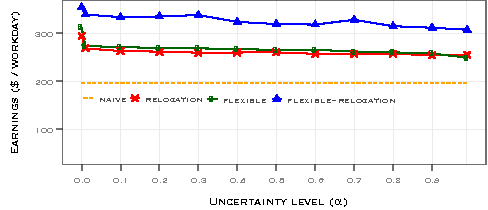
\includegraphics[width=0.65\paperwidth]{figures/uncertainty_evolution.pdf}
	% \caption{Effect of uncertainty}
\end{figure}
\alert{Flexible-Relocation Strategy outperforms all other strategies even in presence of high uncertainty!}
\end{frame}